\documentclass[11pt]{article}

\usepackage[margin=0.75in]{geometry}
\usepackage{amsmath,amssymb}
\usepackage{graphicx}
\usepackage{booktabs}
\usepackage{xcolor}
\usepackage[hidelinks]{hyperref}
\usepackage{titlesec}
\usepackage{float}
\usepackage{subcaption}
\usepackage{listings}

\titleformat{\section}{\large\bfseries}{\thesection}{1em}{}
\titleformat{\subsection}{\bfseries\color{blue!60!black}}{\thesubsection}{1em}{}
\titlespacing*{\section}{0pt}{10pt}{4pt}
\titlespacing*{\subsection}{0pt}{6pt}{3pt}
\setlength{\abovedisplayskip}{5pt}
\setlength{\belowdisplayskip}{5pt}
\captionsetup{font=small, skip=4pt}
\setlength{\intextsep}{6pt}

\lstset{
  language=Python,
  basicstyle=\ttfamily\footnotesize,
  keywordstyle=\color{blue!60!black}\bfseries,
  commentstyle=\color{gray},
  stringstyle=\color{orange!70!black},
  frame=single,
  rulecolor=\color{gray!40},
  backgroundcolor=\color{gray!4},
  columns=fullflexible,
  keepspaces=true,
  showstringspaces=false,
  xleftmargin=4pt, xrightmargin=4pt,
  aboveskip=4pt, belowskip=4pt,
}

\title{\vspace{-0.5in}\Large\bfseries MSAI-635 Assignment 4: Dyna-Q and Dyna-Q+ in a Changing Maze}
\author{Gaurav Prakash \\ UID: 122250130}
\date{\vspace{-0.35in}}

\begin{document}

\maketitle

\section{Problem Formulation}
The environment is a $6 \times 9$ gridworld (0-indexed, row 0 at the top) with start
$S = (5,3)$ and goal $G = (0,8)$. The agent moves up, down, left or right; moves are
deterministic, and a move into a wall or off the grid leaves it in place. The reward is $+1$ for
the transition into $G$ and $0$ otherwise. The task is \emph{continuing}: after reaching $G$ the
agent restarts at $S$ and the clock keeps running, so cumulative reward counts goal visits.
For the first 500 steps a wall covers columns 1--8 of row 3, so the only route passes
through $(3,0)$ and takes 16 steps. At step 500, $(3,8)$ opens, creating a 10-step shortcut
(Figure~\ref{fig:maze}). The old route still works, so the agent receives no signal that
anything changed. The question is whether an agent that has already learned a route will
discover a better one.

\begin{figure}[H]
\centering
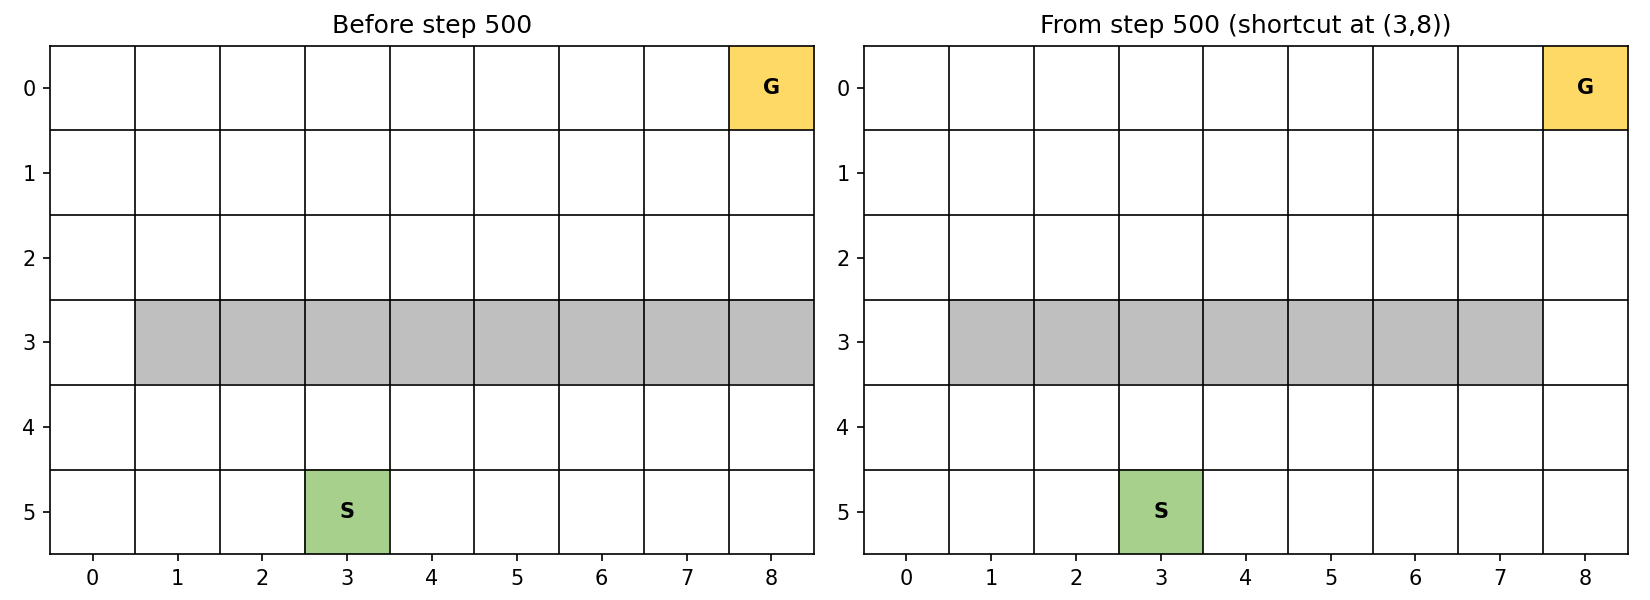
\includegraphics[width=0.78\textwidth]{figures/maze_layouts.png}
\caption{The maze before step 500 (left) and from step 500 on (right). Gray cells are walls; the
only change is that $(3,8)$ opens.}
\label{fig:maze}
\end{figure}

\section{Methodology}

\subsection{Maze environment (\texttt{maze.py})}
\texttt{ChangingMaze} stores $S$, $G$, the current wall set and a global time-step counter.
\texttt{next\_cell(s, a)} returns $s$ unchanged when the target is off the grid or a wall.
\texttt{step(a)} returns (\textit{next state}, \textit{reward}, \textit{reached goal}); on reaching
$G$ it returns $G$ (so the agent treats it as terminal) and moves the agent back to $S$. The
environment switches to the second wall layout itself when its counter reaches 500, so the change
happens at exactly the same step for every agent and run. Self-tests check moves into open cells,
walls and edges, the goal reward and reset, and that $(3,8)$ is closed at step 499 and open at 500.

\subsection{Dyna-Q}
Each real time step Dyna-Q performs (d) a \emph{direct RL} update with one-step
Q-learning,
\[
Q(S,A) \leftarrow Q(S,A) + \alpha\bigl[R + \gamma \max_a Q(S',a) - Q(S,A)\bigr]
\]
(no bootstrap when $S' = G$); (e) \emph{model learning}, storing
$\text{Model}(S,A) = (R, S')$, which is exact because the maze is deterministic; and
(f) \emph{planning}: $n = 10$ times, pick a previously observed $(S,A)$ at random, look up the
model's $(R,S')$ and apply the same update to this \emph{simulated} experience. Actions are
$\varepsilon$-greedy with random tie-breaking, which matters early on when every $Q$ is 0.

\begin{lstlisting}
class DynaQAgent:
    def q_update(self, s, a, r, s2, terminal):          # one-step Q-learning
        target = r if terminal else r + self.gamma * self.q(s2).max()
        self.q(s)[a] += self.alpha * (target - self.q(s)[a])

    def planning_reward(self, s, a, r, t):              # Dyna-Q: the model's reward
        return r

    def plan(self, t):                                  # n simulated updates
        for _ in range(self.n_planning):
            s, a = self.model_keys[self.rng.integers(len(self.model_keys))]
            r, s2, terminal = self.model[(s, a)]
            self.q_update(s, a, self.planning_reward(s, a, r, t), s2, terminal)

    def learn(self, s, a, r, s2, terminal, t):          # one real time step
        self.q_update(s, a, r, s2, terminal)            # (d) direct RL
        self.update_model(s, a, r, s2, terminal, t)     # (e) model learning
        self.plan(t)                                    # (f) planning
\end{lstlisting}

\subsection{Dyna-Q+}
Dyna-Q+ differs in two ways. First, it records when each $(s,a)$ was last executed for real,
with $\tau(s,a)$ the number of steps since then, and \emph{during planning only} uses the reward
$r + \kappa\sqrt{\tau(s,a)}$ with $\kappa = 0.001$; the direct RL update keeps the true reward.
Second, following the footnote to Example 8.3 in Sutton and Barto, the first time a state is visited
all four of its actions enter the model as ``stays in $s$ with reward 0'', last tried at step 0.
Otherwise an untried action would never be sampled in planning and never earn a bonus. The real
transition overwrites the placeholder once the action is taken. Dyna-Q does not use this
initialisation.

\begin{lstlisting}
class DynaQPlusAgent(DynaQAgent):
    def init_state(self, s):                  # first visit: untried actions as self-loops
        if s in self.seen_states:
            return
        self.seen_states.add(s)
        for a in range(self.n_actions):
            if (s, a) not in self.model:
                self.model_keys.append((s, a))
                self.model[(s, a)] = (0.0, s, False)
                self.last_tried[(s, a)] = 0  # tau counted from the start of the run

    def update_model(self, s, a, r, s2, terminal, t):
        self.init_state(s)
        super().update_model(s, a, r, s2, terminal, t)   # real transition overwrites
        self.last_tried[(s, a)] = t                      # reset tau for (s, a)

    def planning_reward(self, s, a, r, t):    # bonus applied only in planning
        return r + self.kappa * np.sqrt(t - self.last_tried[(s, a)])
\end{lstlisting}

\noindent Unit tests in \texttt{agents.py} check the Q-update by hand, that Dyna-Q stores only
real transitions, the four Dyna-Q+ placeholders per new state, the $\tau$ bookkeeping, the bonus
value ($\kappa\sqrt{100} = 0.01$), and that the direct RL update receives no bonus.

\section{Experimental Setup}
Both agents use $\gamma = 0.95$, $\alpha = 1.0$, $\varepsilon = 0.1$ and $n = 10$; Dyna-Q+ adds
$\kappa = 0.001$. \texttt{experiments.py} runs each agent for 3000 real time steps on a fresh
maze whose shortcut opens at step 500, with the same 100 seeds (0--99) for both agents, and
averages over the runs. Each run records the cumulative reward after every step, and every
completed trip from $S$ to $G$ with its length and whether it passed through $(3,8)$. Runs are
also split by whether they had reached $G$ before the change. This matters because, until the
first goal, all rewards are 0 and planning has nothing to propagate. The first goal arrives at a
median step of 510 for Dyna-Q (442 for Dyna-Q+), so in about half of the runs the shortcut opens
before any route is known, and only the remaining runs really test adaptation.

\section{Results}
Both curves in Figure~\ref{fig:cum} are almost identical up to about step 600. After that
Dyna-Q+ climbs faster and finishes with 179.4 cumulative reward against 155.3 for Dyna-Q
(Table~\ref{tab:main}). Figure~\ref{fig:usage} shows why: Dyna-Q+'s share of trips through the
shortcut rises to about 90\%, while Dyna-Q's levels off near 55\%.

\begin{figure}[H]
\centering
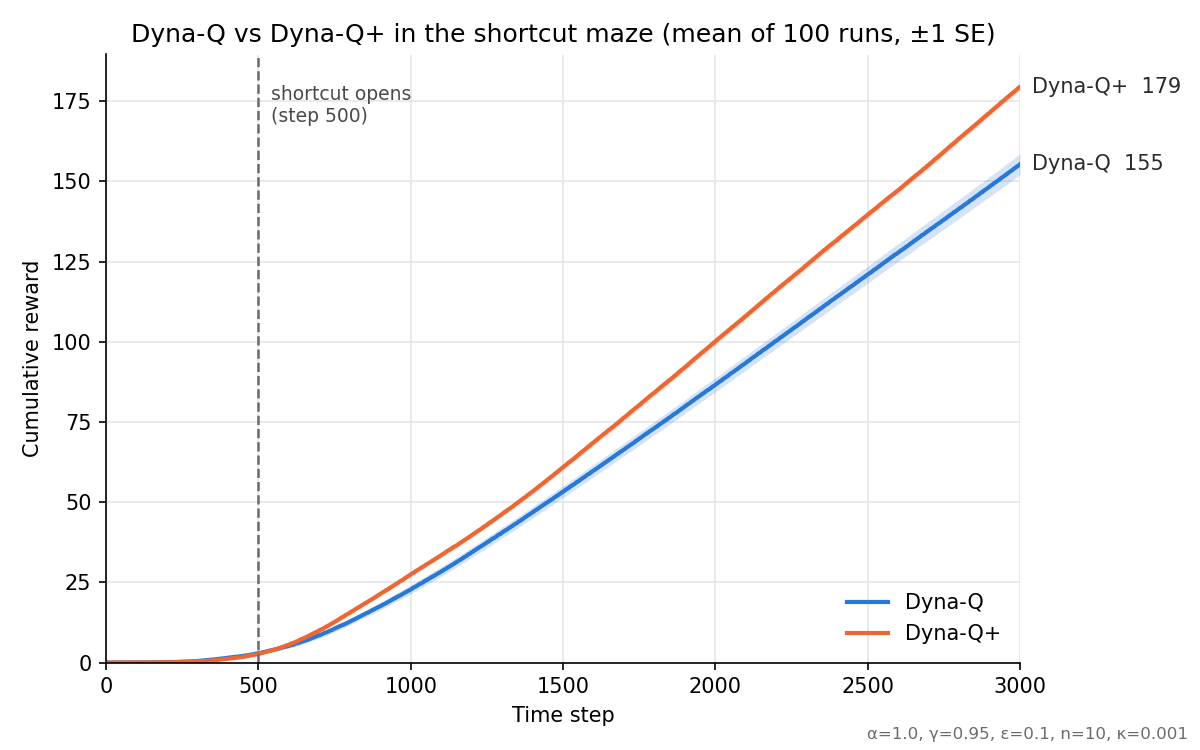
\includegraphics[width=0.72\textwidth]{figures/cumulative_reward_change500_steps3000_runs100.png}
\caption{Cumulative reward vs.\ time step, mean of 100 runs per agent with $\pm 1$ standard-error
bands. The dashed line marks step 500, when the shortcut opens.}
\label{fig:cum}
\end{figure}

\begin{figure}[H]
\centering
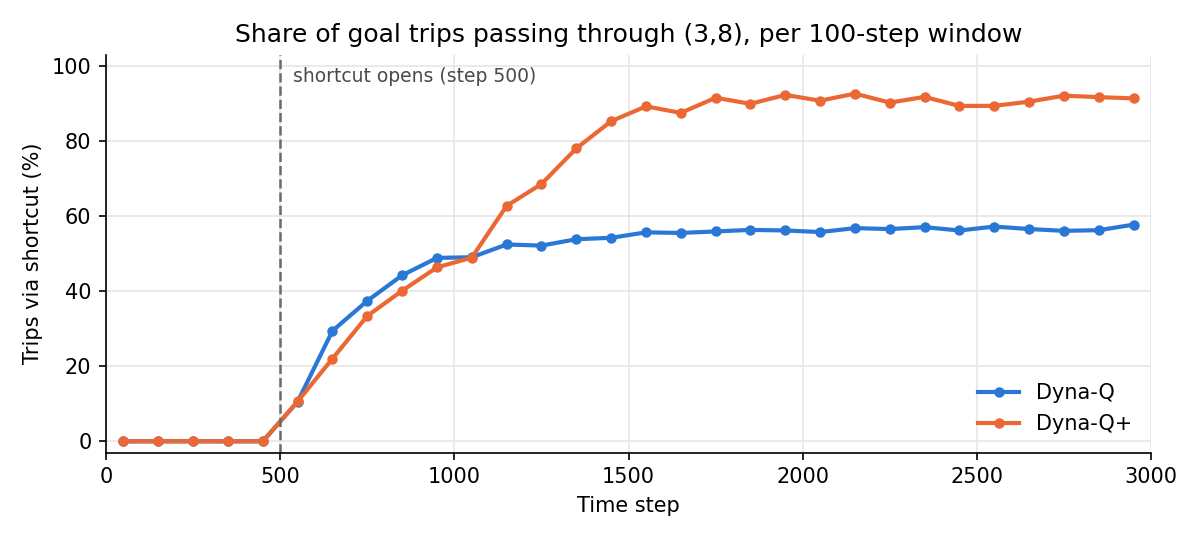
\includegraphics[width=0.72\textwidth]{figures/shortcut_usage_change500_steps3000_runs100.png}
\caption{Share of completed trips passing through $(3,8)$, pooled over the 100 runs, per 100-step
window.}
\label{fig:usage}
\end{figure}

\begin{table}[H]
\centering
\small
\begin{tabular}{lccccc}
\toprule
 & \multicolumn{3}{c}{cumulative reward} & \multicolumn{2}{c}{last 500 steps} \\
\cmidrule(lr){2-4}\cmidrule(lr){5-6}
agent & step 500 & step 3000 & gained after change & trips via $(3,8)$ & mean trip length \\
\midrule
Dyna-Q  & 2.9 & 155.3 & $152.4 \pm 3.4$ & 45\% & 11.6 / 18.5$^\dagger$ \\
Dyna-Q+ & 2.7 & 179.4 & $176.8 \pm 1.0$ & 91\% & 12.6 \\
\bottomrule
\end{tabular}
\caption{Mean over 100 runs ($\pm$ one standard error). Optimal trip length: 16 steps on the
old route, 10 via the shortcut. $^\dagger$Dyna-Q runs on the shortcut / on the old route.}
\label{tab:main}
\end{table}

\begin{table}[H]
\centering
\small
\begin{tabular}{lcc}
\toprule
runs & Dyna-Q switched & Dyna-Q+ switched \\
\midrule
had reached $G$ before step 500 & 5 / 47 (11\%) & 66 / 66 (100\%) \\
had not reached $G$ yet         & 40 / 53 (75\%) & 34 / 34 (100\%) \\
\bottomrule
\end{tabular}
\caption{Runs that ended on the shortcut (more than half of their last-500-step trips through
$(3,8)$), split by whether the old route was known when the shortcut opened.}
\label{tab:split}
\end{table}

\noindent Table~\ref{tab:split} separates real adaptation from luck. Dyna-Q runs that already
knew the old route almost never switch (11\%). Most Dyna-Q runs that do use the shortcut had not
yet found the goal at step 500, so they found the shortcut first simply because it was there.
Every Dyna-Q+ run switches, whether or not it knew the old route. This split also explains
Dyna-Q's wider error band: its runs fall into two groups with very different reward rates.

\section{Discussion}

\subsection{Conceptual question: why does Dyna-Q+ outperform Dyna-Q after the maze changes?}
After step 500 both agents' models are wrong: they say that moving up from $(4,8)$ hits the
wall, or that action was never tried. \textbf{Dyna-Q} has no reason to question this. Its model
is corrected only by real experience, and its planning keeps replaying the stale transitions,
which confirms the old route ten times per step. Its greedy policy follows the left-hand route
and rarely visits the right side of the maze. Its only exploration is $\varepsilon$-greedy, which
is \emph{undirected}: reaching $(4,8)$ and choosing ``up'' would take several unlikely random
moves in a row, each pulled back by the greedy policy. Because the old route never gets worse,
nothing forces a re-check, and only 5 of 47 runs that knew the old route ever switched.

\textbf{Dyna-Q+} rewards checking. Each pair not executed for $\tau$ steps earns a planning bonus
$\kappa\sqrt{\tau}$ that keeps growing, and the pairs near the shortcut are exactly the ones the old
route never executes. Planning propagates the bonus backwards like a real reward, so actions
\emph{leading toward} those neglected states also gain value, until the greedy policy walks to
$(4,8)$ and tries ``up''. A rough estimate of the timing: the self-loop ``up'' at $(4,8)$ has
planned value $\kappa\sqrt{\tau} + \gamma V(4,8)$, against about $V(4,8)$ for the best real
action. With $V(4,8) \approx 0.95^{19} \approx 0.38$ (20 steps to $G$ on the old route), trying
the wall again becomes greedy once $\kappa\sqrt{\tau} > (1-\gamma)V(4,8) \approx 0.019$, i.e.\
after about $\tau \approx 360$ steps. This matches the time scale on which Dyna-Q+'s shortcut use
rises in Figure~\ref{fig:usage}. Once tried, the real transition ``up at $(4,8) \to (3,8)$''
overwrites the stale model entry, and ten planning updates per step quickly spread the value of
the shorter path. In short, Dyna-Q+ assumes that anything not checked recently may have
changed. Dyna-Q assumes its model stays correct until experience proves otherwise, and here that
never happens.

\subsection{Exploration versus exploitation}
The bonus has a cost. Dyna-Q runs on the shortcut average 11.6 steps per trip, while Dyna-Q+
averages 12.6, and about 9\% of its trips still avoid $(3,8)$, because it keeps making small
detours to re-check moves it has not tried lately. Dyna-Q exploits its model fully and is
slightly more efficient \emph{while the model is correct}, but loses heavily once it is wrong.
Dyna-Q+ gives up a little reward all the time to detect change, which pays off here (39.8 vs.\
34.4 reward over the last 500 steps). $\kappa$ sets the price: a larger $\kappa$ re-checks sooner
but wastes more steps in a stationary world, and $\kappa \to 0$ gives back Dyna-Q. Directed
exploration also helps before the change: Dyna-Q+ reaches the goal for the first time at a median
step of 442, against 510 for Dyna-Q.

\subsection{Real experience, simulated experience and planning}
Only real experience can correct the model; planning makes the most of the model the agent
already has. With $n = 10$, each real step drives eleven $Q$ updates, so once either agent finds
the goal it learns a full route within a few trips rather than the many episodes Q-learning would
need, at a computational cost that grows linearly in $n$. The same efficiency makes Dyna-Q's
failure worse, since planning with a stale model reinforces the old route. Dyna-Q+ keeps the
efficiency and uses the bonus to decide where to collect new real experience.

\section{Conclusions}
Dyna-Q and Dyna-Q+ were implemented and compared over 100 runs each under identical
conditions. After the shortcut opens at step 500, Dyna-Q+ ends with 179.4 cumulative reward
against 155.3 for Dyna-Q. Every Dyna-Q+ run moves to the 10-step shortcut, while Dyna-Q runs
that already knew the old route switch only 11\% of the time. Dyna-Q's planning keeps replaying a
model that is out of date, and its $\varepsilon$-greedy exploration is too undirected to fix it.
Dyna-Q+'s bonus $\kappa\sqrt{\tau}$ makes long-neglected actions attractive during planning, so
the agent returns, observes the new transition and updates its model, at the cost of about one
extra step per trip.

\end{document}
